\subsection{Experimental setup}
We adopt the data and evaluation pipeline from the TTRL codebase \citep{zuo2025ttrl}, which is built on the VERL framework \citep{sheng2024hybridflow}.
The final answer of the language model is the string inside the last \emph{\textbackslash boxed\{\}}.

\paragraph{Implementation details.} 
We use hyperparameters similar to those in TTRL \citep{zuo2025ttrl} and report them here for completeness. 
A cosine learning rate schedule is applied, with a peak value of $5 \times 10^{-7}$, and the AdamW optimiser is used for the policy model with a learning rate of $9 \times 10^{-6}$. 
The KL-regularisation parameter in the RL objective is set to $0.001$.

We sample 64 responses per prompt using a temperature of $0.6$ ($1.0$ for Qwen2.5-Math models) for voting-based label estimation, and downsample $32$ responses per prompt for training. The maximum generation length is fixed at $3072$ tokens for all models. The number of episodes is set to $80$, $30$, and $10$ for AIME 2024, AMC, and MATH-500, respectively, reflecting dataset size. We also apply early stopping with a tolerance of $5\times 10^{-3}$ and a patience of $10$ iterations, evaluated on both metrics (pass@1 and majority).

All other hyperparameters not explicitly mentioned here are set to their default values in the VERL framework.
For the TTRL \citep{zuo2025ttrl} baseline, we adopt the hyperparameters reported in the paper.


\paragraph{Evaluation details.}
We also set the maximum generation length to $3072$ tokens during evaluation.
Following \citet{zuo2025ttrl}, we report the pass@1 score using non-zero temperature
sampling. Specifically, for each prompt $pr$, we generate $N=16$ responses using a
temperature of $0.6$ and a top-p value of $0.95$. 
The pass@1 score is then computed as
$$
\text{pass@1}= \frac{1}{QN}\sum_{pr}\sum_{i=1}^N \mathbf{1}\{X_i(pr)=\text{correct}\},
$$
where $X_i(pr)$ denotes the $i$-th generated response for prompt $pr$ and $Q$ is the total number of prompts.

We also report majority vote accuracy, which indicates whether the most frequent answer among the $N = 16$ responses per prompt matches the ground truth
$$
\text{majority}= \frac{1}{Q}\sum_{pr} \mathbf{1}\{\text{majority vote}(X_1(pr), \dots, X_N(pr))=\text{correct}\}.
$$

\paragraph{Computation time.}
All experiments were conducted on 8$\times$H100 Nvidia GPUs, each with 96GB of memory.


\subsection{Additional results}\label{app:subsec_additional_results}
Table~\ref{tab:test-time-training-results-pass1-format-score} expands upon the results presented in Table~\ref{tab:test-time-training-results}. 
It reports the pass@1 performance for both the score and the format score before and after applying test-time training with our proposed reward functions. 
We observe that, for Qwen2.5 models, the improvement in score is notably larger than that in format score, suggesting that test-time training effectively uncovers latent knowledge already present in the model rather than merely correcting format errors.
In contrast, for the Llama-3.1-8B model, we hypothesise that the mode of the model's final answer distribution does not coincide with the true answer, therefore, test-time training incorrectly shifts the model's output distribution. That is, the model lacks the necessary mathematical knowledge, and our test-time training strategies serve to reveal rather than create new knowledge.
Table~\ref{tab:test-time-training-results-majority-format-score} presents analogous results for majority vote accuracy, leading to similar conclusions.

\begin{table}[b!]
\caption{Comparison of pass@1 performance for the score and format score (using 16 samples per prompt) before and after applying test-time training.}
\label{tab:test-time-training-results-pass1-format-score}
\begin{center}
\footnotesize
\begin{tabular}{lcccccc}
\toprule
     & \multicolumn{2}{c}{\textbf{AIME}} & \multicolumn{2}{c}{\textbf{AMC}} & \multicolumn{2}{c}{\textbf{Math\scriptsize-500\footnotesize}} \\
\midrule
     & \textbf{Score} & \textbf{Format score}  & \textbf{Score} & \textbf{Format score}  & \textbf{Score} & \textbf{Format score}\\
\midrule
\textbf{Qwen2.5-7B} &9.4&  84.6 &31.2& 84.6 &59.1& 90.2\\
\\
\multirow{2}{*}{SNR}  &23.3& 100.0 &51.8& 99.5 &80.3 &98.9 \\
  &\textcolor{green}{+13.9}  & \textcolor{green}{+15.4}   &\textcolor{green}{+20.6}& \textcolor{green}{+14.9}&\textcolor{green}{+21.2}& \textcolor{green}{+8.7} \\
 \\
\multirow{2}{*}{Entropy}  &20.0& 100.0 &49.2& 99.5 &77.6& 100.0\\
 &\textcolor{green}{+10.6}& \textcolor{green}{+15.4} &\textcolor{green}{+18.0}& \textcolor{green}{+14.9} &\textcolor{green}{+18.5}& \textcolor{green}{+9.8} \\
\midrule
\textbf{Llama-3.1-8B} & 4.4& 60.0 & 21.8 & 72.0 &48.2& 83.8\\
\\
\multirow{2}{*}{SNR}  &13.4& 99.6 &29.3& 100.0 &59.2& 100.0 \\
 &\textcolor{green}{+9.0}& \textcolor{green}{+39.6} &\textcolor{green}{+7.5}& \textcolor{green}{+28.0}&\textcolor{green}{+11.0}& \textcolor{green}{+16.2} \\
 \\
\multirow{2}{*}{Entropy}    &13.3& 99.8 &27.0& 100.0 &55.4& 100.0\\
  &\textcolor{green}{+8.9}& \textcolor{green}{+39.8}&\textcolor{green}{+5.2}&  \textcolor{green}{+28.0} &\textcolor{green}{+7.2}& \textcolor{green}{+16.2}\\
\midrule
\textbf{Qwen2.5-Math-7B}  &10.6&  73.5 &31.0& 85.4 &47.1& 90.2\\
\\
\multirow{2}{*}{SNR}   & 36.7& 85.4 &65.0& 88.8 &84.5& 97.5 \\
  &\textcolor{green}{+26.1}& \textcolor{green}{+11.9}   &\textcolor{green}{+34.0}& \textcolor{green}{+3.4} &\textcolor{green}{+37.4}& \textcolor{green}{+7.3}   \\
 \\
\multirow{2}{*}{Entropy}    &38.3& 97.5 &65.4& 99.9  &82.4 & 99.3\\
  &\textcolor{green}{+27.7}& \textcolor{green}{+24.0} &\textcolor{green}{+34.4}&  \textcolor{green}{+14.5} &\textcolor{green}{+35.3}&  \textcolor{green}{+9.1}\\
\midrule
\textbf{Qwen2.5-Math-1.5B}  & 7.1& 74.2 & 28.1 & 80.1 &31.4 & 66.4\\
\\
\multirow{2}{*}{SNR}  &16.3 & 91.9& 45.4& 92.2& 72.0 & 97.7\\
 &\textcolor{green}{+9.2}& \textcolor{green}{+17.7} &\textcolor{green}{+17.3}& \textcolor{green}{+12.1} &\textcolor{green}{+40.6}& \textcolor{green}{+11.3} \\
 \\
\multirow{2}{*}{Entropy} &15.6  & 88.3 &45.9& 96.2 &70.8& 98.1\\
  &\textcolor{green}{+8.5}& \textcolor{green}{+14.1}&\textcolor{green}{+17.8}& \textcolor{green}{+16.1} &\textcolor{green}{+39.4}& \textcolor{green}{+11.7}\\
\bottomrule
\end{tabular}
\end{center}
\end{table}
\normalsize


\begin{table}[ht!]
\caption{Comparison of majority vote accuracy for the  score and format score (using 16 samples per prompt) before and after applying test-time training.}
\label{tab:test-time-training-results-majority-format-score}
\begin{center}
\footnotesize
\begin{tabular}{lcccccc}
\toprule
     & \multicolumn{2}{c}{\textbf{AIME}} & \multicolumn{2}{c}{\textbf{AMC}} & \multicolumn{2}{c}{\textbf{Math\scriptsize-500\footnotesize}} \\
\midrule
     & \textbf{Score} & \textbf{Format score}  & \textbf{Score} & \textbf{Format score}  & \textbf{Score} & \textbf{Format score}\\
\midrule
\textbf{Qwen2.5-7B} & 16.7 & 72.8 &41.8  & 79.6 &73.5 &  93.4\\
\\
\multirow{2}{*}{SNR} &23.3& 100.0 &51.2&100.0 &81.0& 98.9\\
 &\textcolor{green}{+6.6} & \textcolor{green}{+27.2}  &\textcolor{green}{+9.4} & \textcolor{green}{+20.4}&\textcolor{green}{+7.5} & \textcolor{green}{+5.5} \\
 \\
\multirow{2}{*}{Entropy} &20.0& 100.0 &49.4&100.0 &79.0& 100.0\\
 & \textcolor{green}{+3.3}& \textcolor{green}{+27.2}   &\textcolor{green}{+7.6} & \textcolor{green}{+20.4}&\textcolor{green}{+5.5} & \textcolor{green}{+6.6}\\
\midrule
\textbf{Llama-3.1-8B} &4.6& 26.8 &27.4& 53.4 &57.7 & 77.2\\
\\
\multirow{2}{*}{SNR}  &13.3 & 99.8 &28.6& 100.0&60.3& 100.0\\
& \textcolor{green}{+8.7} & \textcolor{green}{+73.0}  &\textcolor{green}{+1.2}& \textcolor{green}{+46.6} &\textcolor{green}{+2.6} & \textcolor{green}{+22.8}\\
 \\
\multirow{2}{*}{Entropy}   & 13.3 & 100.0 & 29.3 & 100.0&57.6& 100.0\\
&\textcolor{green}{+8.7}& \textcolor{green}{+73.2} &\textcolor{green}{+1.9}& \textcolor{green}{+46.6} & \textcolor{red}{-0.1} & \textcolor{green}{+22.8}\\
\midrule
\textbf{Qwen2.5-Math-7B} &16.5& 56.3 &41.5 & 78.4 &59.5& 87.8\\
\\
\multirow{2}{*}{SNR}  &37.8& 77.9 &67.2 & 87.9 &85.7& 99.5\\
&\textcolor{green}{+21.3} & \textcolor{green}{+21.6} &\textcolor{green}{+25.7}& \textcolor{green}{+9.5}&\textcolor{green}{+26.2} & \textcolor{green}{+11.7} \\
 \\
\multirow{2}{*}{Entropy}   &36.7& 97.3 & 66.1& 100.0&84.3 & 99.5\\
&\textcolor{green}{+20.2} & \textcolor{green}{+41.0}  &\textcolor{green}{+24.6} & \textcolor{green}{+22.6} &\textcolor{green}{+24.8} & \textcolor{green}{+11.7} \\
\midrule
\textbf{Qwen2.5-Math-1.5B} &11.7& 60.0 &37.2&  70.8 &36.5 & 57.4\\
\\
\multirow{2}{*}{SNR}  &23.7 & 90.5 &53.3&  90.9&78.9 & 97.8\\
& \textcolor{green}{+12.0} &\textcolor{green}{+30.5} & \textcolor{green}{+16.1}&   \textcolor{green}{+20.1}&\textcolor{green}{+42.4}& \textcolor{green}{+40.4}\\
 \\
\multirow{2}{*}{Entropy}  &23.2  &  81.3 &52.8& 95.7 &77.4 & 98.2\\
 &\textcolor{green}{+11.5} & \textcolor{green}{+21.3} &\textcolor{green}{+15.6}&   \textcolor{green}{+24.9} &\textcolor{green}{+40.9} & \textcolor{green}{+40.8}\\
\bottomrule
\end{tabular}
\end{center}
\end{table}
\normalsize

Table~\ref{tab:ratio_adaptive_sampling_pre_post_trained} provides evidence that the model becomes more confident in its outputs after applying test-time training strategies.
Specifically, the required number of samples for the MMC stopping rule, denoted as $N_{\text{adaptive}}$ is lower after test-time training compared to the pre-trained model.

The relationship between $N_{\text{adaptive}}$ and $N_{\text{budget}}$ can be accurately modelled by a linear regression of the form $N_{\text{adaptive}} = \alpha + \beta N_{\text{budget}}$ with a coefficient of determination $R^2$ very close to 1. We therefore report the estimated value of $\beta$ obtained via least squares fitting.
Since $0\leq N_{\text{adaptive}}\leq N_{\text{budget}}$, it follows that $\beta\leq1$. 

We observe that the estimated slope for the pre-trained model, $\hat\beta_{\text{pre}}$, is larger than that of the test-time trained model, $\hat\beta_{\text{post}}$. This reduction is particularly pronounced for the smaller 1.5B model, suggesting that larger models experience diminishing returns from test-time training.

These results are consistent with the larger increase in the estimated ${\text{SNR}}(\Delta_{j^\star_n})$ observed during training.
Recall from (\ref{eq:expected_number_samples}) that the required number of samples for the MMC stopping rule is approximately inversely proportional to the ${\text{SNR}}(\Delta_{j^\star_n})$. 
Figure~\ref{fig:evolution_during_training} shows the evolution of the estimated ${\text{SNR}}(\Delta_{j^\star_n})$ when using SNR-based rewards, as well as the negative entropy when training with entropy-based rewards, measured on the training dataset. We also include the evolution of the pass@1 performance on the validation dataset.


\begin{table}[ht!]
\caption{Regression coefficients from fitting the required number of samples under the MMC stopping rule as a function of the budget, ${N}_{\text{adaptive}} = \alpha + \beta {N}_{\text{budget}}$, for $\varepsilon = 0.1$ and $0.4$. Results contrast the pre-trained model with the model after test-time training using SNR-based rewards.}
\label{tab:ratio_adaptive_sampling_pre_post_trained}
\begin{center}
\footnotesize
\begin{tabular}{ccccccccc}
\toprule
  & \multicolumn{2}{c}{\textbf{Qwen2.5-Math-7B} }&\multicolumn{2}{c}{\textbf{Qwen2.5-Math-1.5B}} &\multicolumn{2}{c}{\textbf{Qwen2.5-7B}}&\multicolumn{2}{c}{\textbf{Llama-3.1-8B}}\\
\cmidrule(lr){2-3}
\cmidrule(lr){4-5}
\cmidrule(lr){6-7}
\cmidrule(lr){8-9}
 $\bm \varepsilon$ &0.1&0.4 & 0.1&0.4& 0.1&0.4& 0.1&0.4\\
\midrule
$\bm{\hat\beta}_{\text{pre}}$ pre-trained model  &0.725& 0.711&0.848 &0.798 & 0.627& 0.589& 0.645& 0.590\\
\\
$\bm{\hat\beta}_{\text{post}}$ test-time trained model &0.631 & 0.568& 0.570& 0.533 & 0.472&0.392& 0.564& 0.488\\
\\
$\nabla = \bm{\hat\beta}_{\text{pre}}-\bm{\hat\beta}_{\text{post}}$ & 0.094& 0.143& 0.237&0.265& 0.155& 0.197& 0.081& 0.102\\
\bottomrule
\end{tabular}
\end{center}
\end{table}
\normalsize



\begin{figure}[h!]
  \centering
  \begin{subfigure}{0.98\textwidth}
      \centering
      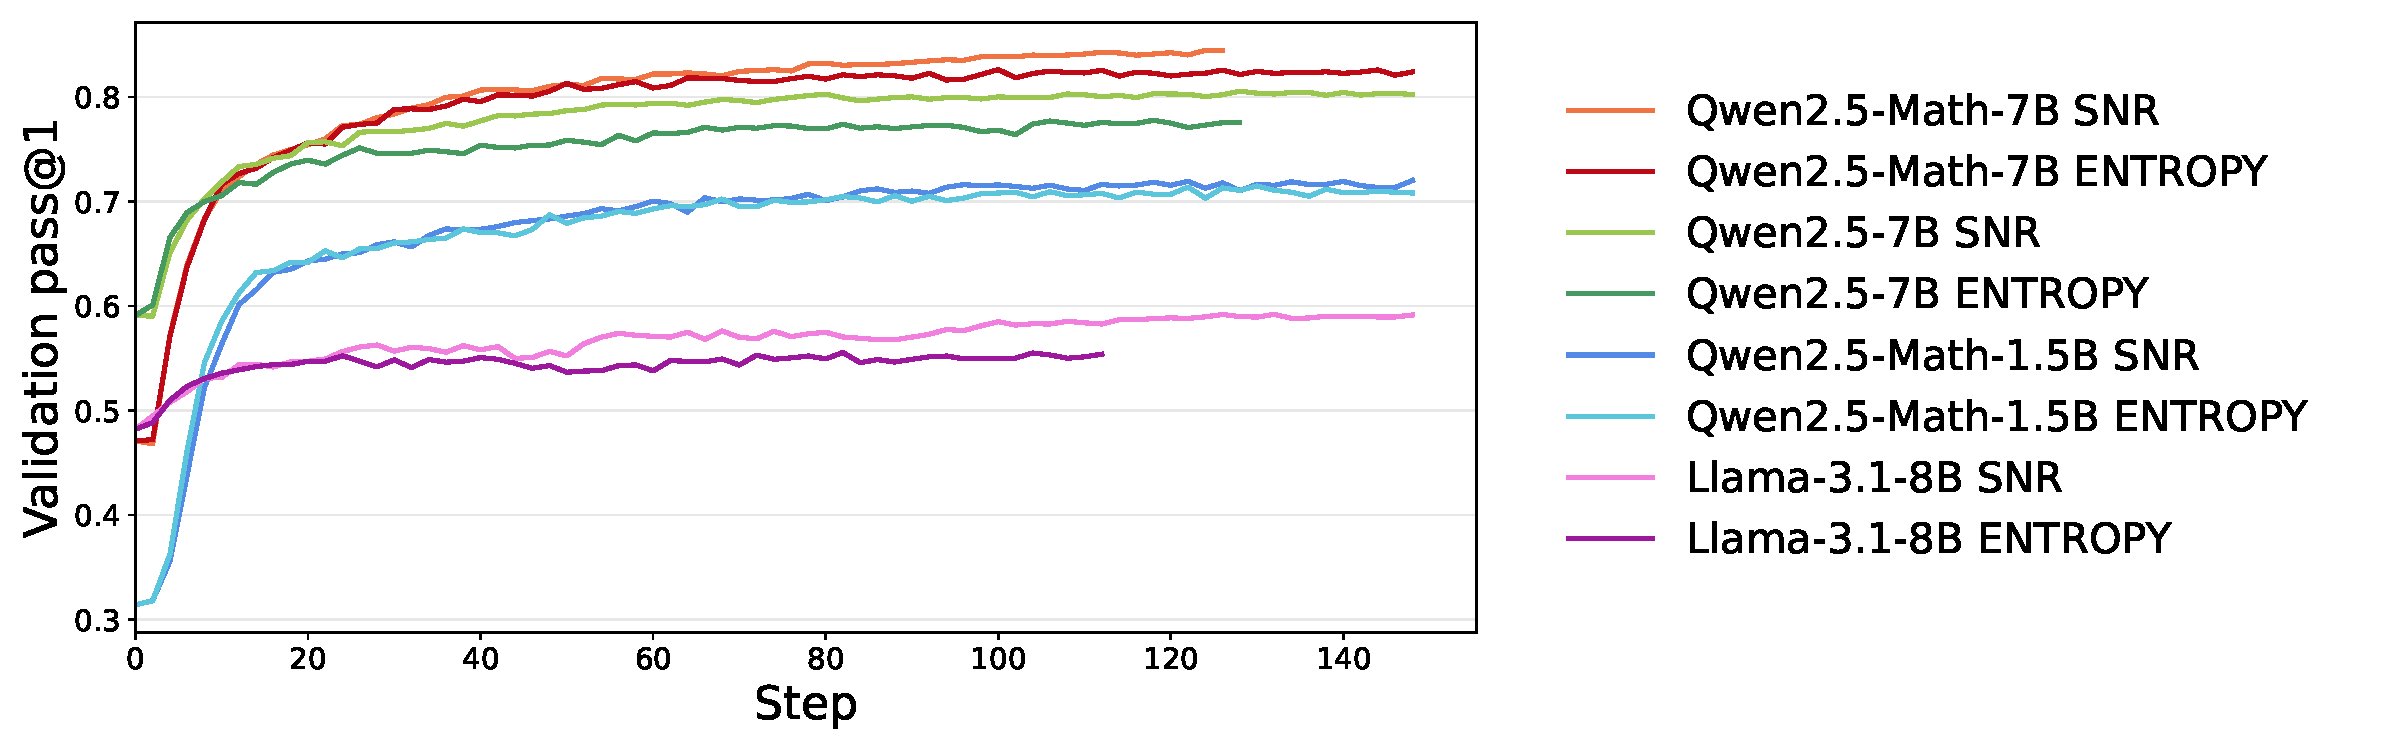
\includegraphics[width=\textwidth]{figs/plot_pass1_validation.pdf}
      \label{fig:evolution_validation_pass@1}
  \end{subfigure}
  \vfill
  \begin{subfigure}{0.49\textwidth}
      \centering
      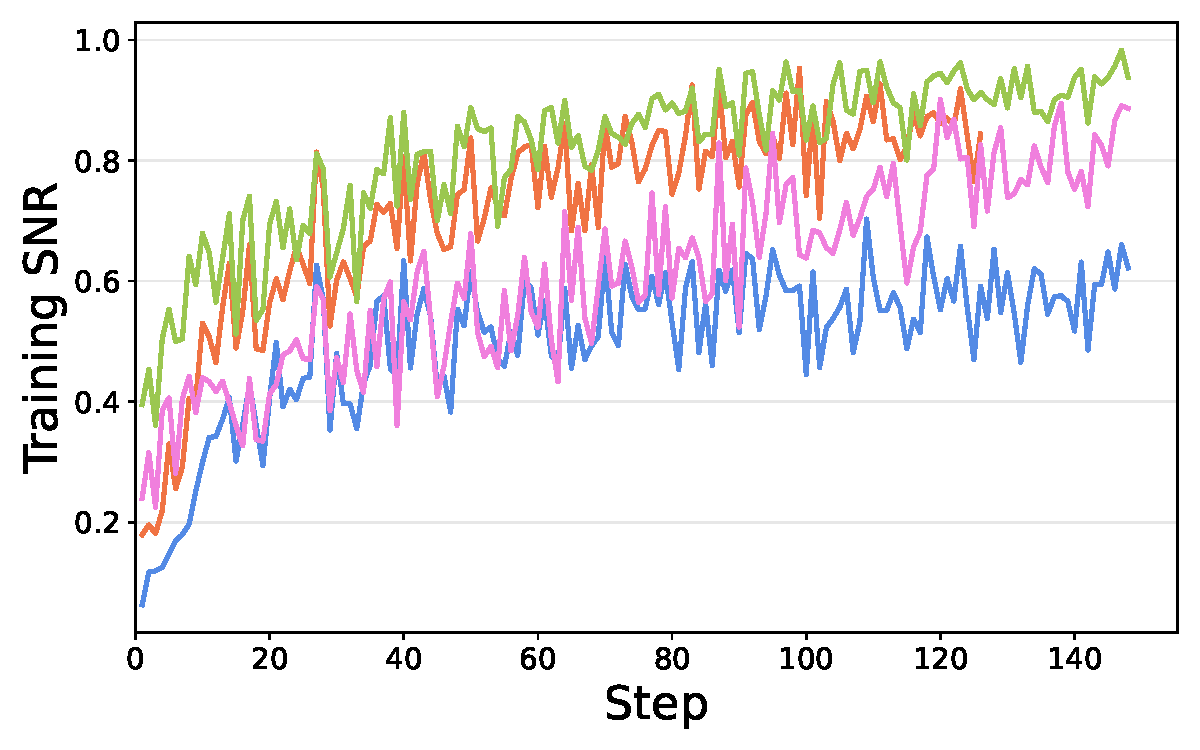
\includegraphics[width=\textwidth]{figs/plot_training_SNR.pdf}
      \label{fig:evolution_training_snr}
  \end{subfigure}
  \hfill
  \begin{subfigure}{0.49\textwidth}
      \centering
      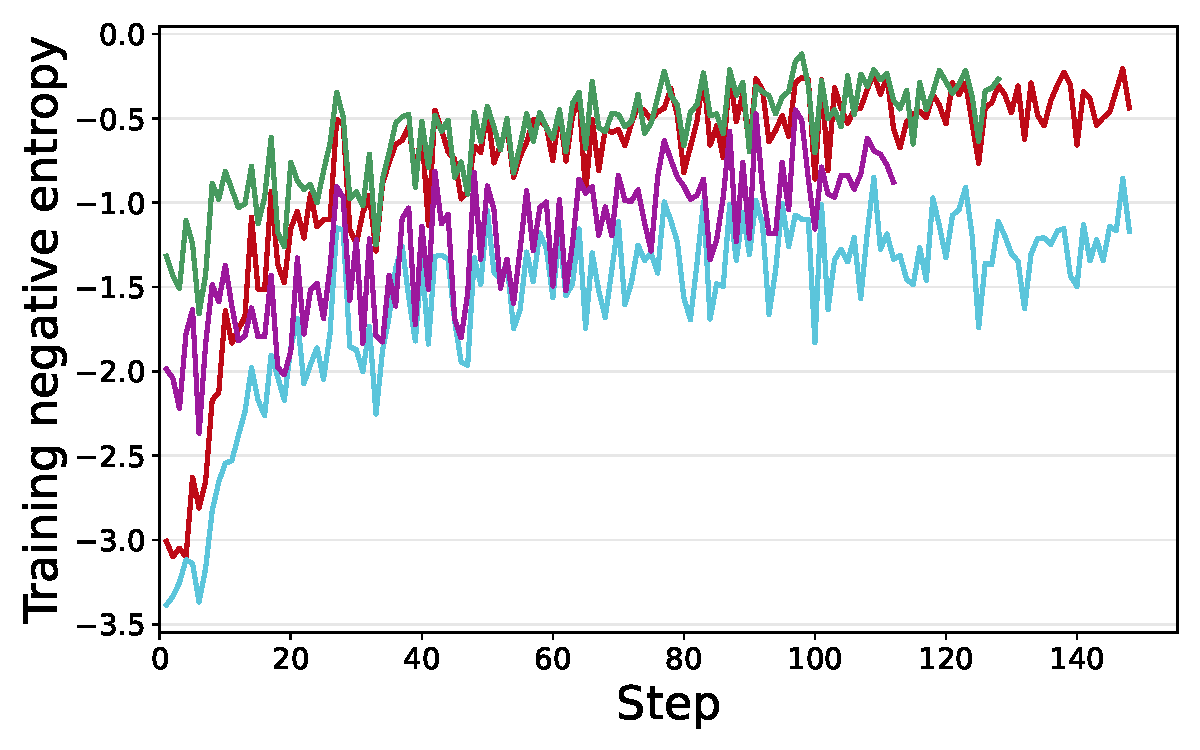
\includegraphics[width=\textwidth]{figs/plot_training_negative_entropy.pdf}
      \label{fig:evolution_training_negative_entropy}
  \end{subfigure}
  \caption{Evolution of different training and validation metrics on the MATH-500 dataset.}
  \label{fig:evolution_during_training}
\end{figure}


Finally, Figures \ref{fig:violin_plots_NO_ground_truth_01}-\ref{fig:violin_plots_SNR_ground_truth_04} provide a detailed analysis, for each difficulty level in the MATH-500 dataset, of the distributions of the estimated lower bound on the probability $\mathbb{P}[\widehat{c}_n= c^\star]$, as well as the estimated ${\text{SNR}}(\Delta_{j^\star_n})$ when applying the MMC adaptive sampling scheme under two confidence levels, $\varepsilon = 0.1$ and $0.4$. 
The lower bound estimates of $\mathbb{P}[\widehat{c}_n = c^\star]$ (Figures \ref{fig:violin_plots_NO_ground_truth_01}, \ref{fig:violin_plots_NO_ground_truth_04}) are computed using a Beta approximation (see Appendix \ref{app:subsec_estimator_proability} for details).
Results are reported after test-time training with SNR-based rewards.
The SNR plots (Figures~\ref{fig:violin_plots_SNR_ground_truth_01}, \ref{fig:violin_plots_SNR_ground_truth_04}) further illustrate how SNR can serve as a label-free estimator of problem difficulty.


\begin{figure}[h!]
  \centering
  \begin{subfigure}{0.49\textwidth}
      \centering
      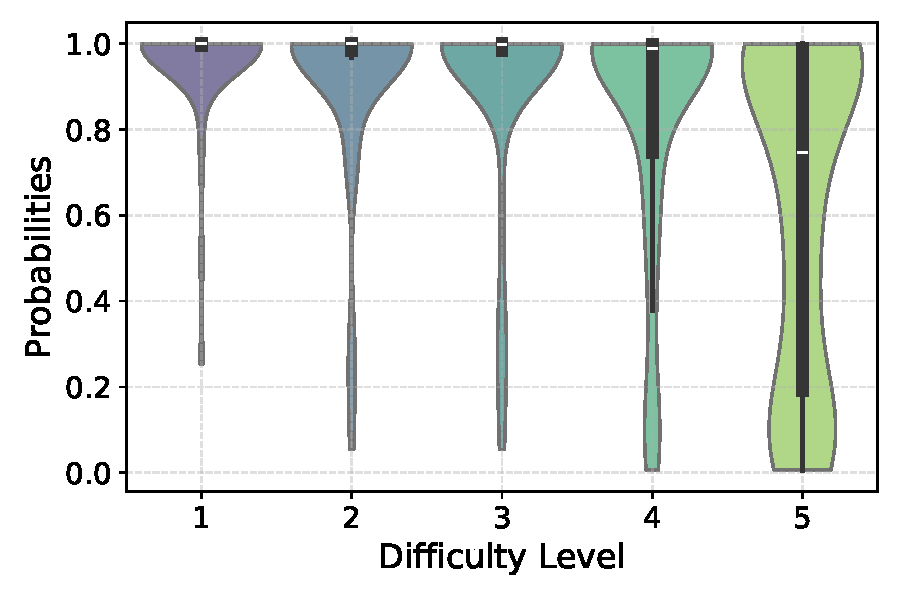
\includegraphics[width=\textwidth]{figs/QWEN-MATH-1.5B_violin_maj10_probability_adaptive_01_NO_ground_truth.pdf}
      \caption{Qwen2.5-Math-1.5B, $N_{\text{budget}}=10$.}
      \label{fig:QWEN-MATH-1.5B_budget_10_NO_01}
  \end{subfigure}
  \hfill
  \begin{subfigure}{0.49\textwidth}
      \centering
      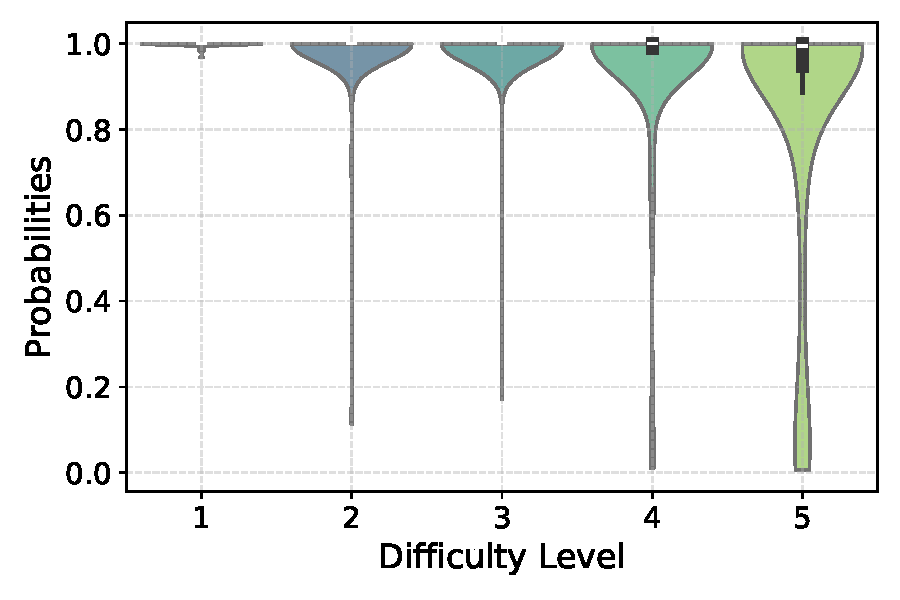
\includegraphics[width=\textwidth]{figs/QWEN-MATH-7B_violin_maj10_probability_adaptive_01_NO_ground_truth.pdf}
        \caption{Qwen2.5-Math-7B, $N_{\text{budget}}=10$.}
      \label{fig:QWEN-MATH-7B_budget_10_NO_01}
  \end{subfigure}
  \vfill
  \begin{subfigure}{0.49\textwidth}
      \centering
      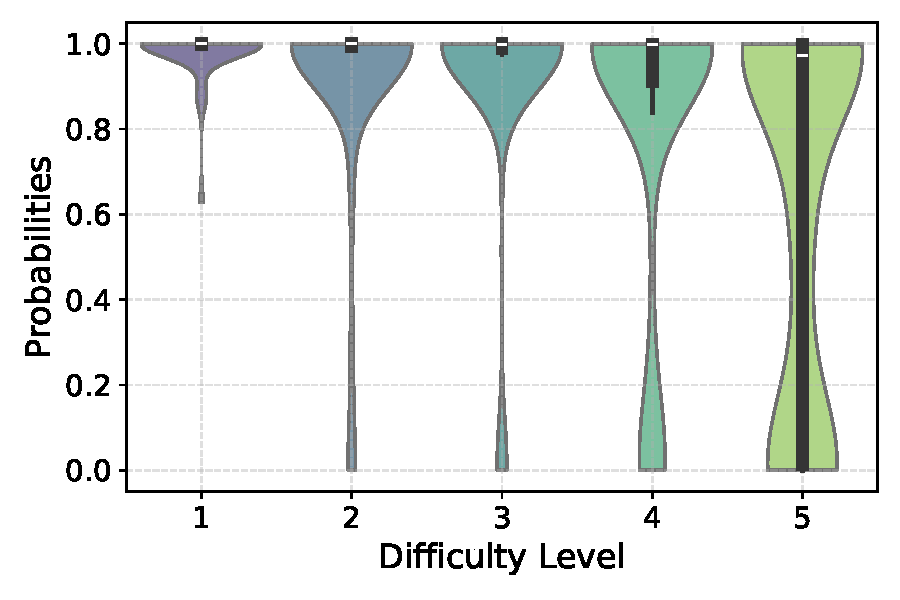
\includegraphics[width=\textwidth]{figs/QWEN-MATH-1.5B_violin_maj50_probability_adaptive_01_NO_ground_truth.pdf}
        \caption{Qwen2.5-Math-1.5B, $N_{\text{budget}}=50$.}
      \label{fig:QWEN-MATH-1.5B_budget_50_NO_01}
  \end{subfigure}
  \hfill
  \begin{subfigure}{0.49\textwidth}
      \centering
      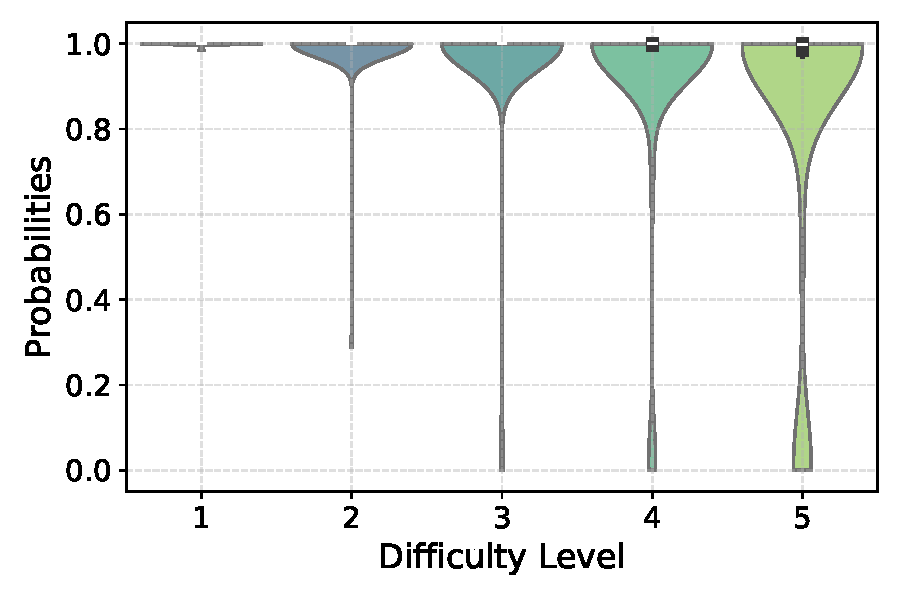
\includegraphics[width=\textwidth]{figs/QWEN-MATH-7B_violin_maj50_probability_adaptive_01_NO_ground_truth.pdf}
        \caption{Qwen2.5-Math-7B, $N_{\text{budget}}=50$.}
      \label{fig:QWEN-MATH-7B_budget_50_NO_01}
  \end{subfigure}
  \vfill
  \begin{subfigure}{0.49\textwidth}
      \centering
      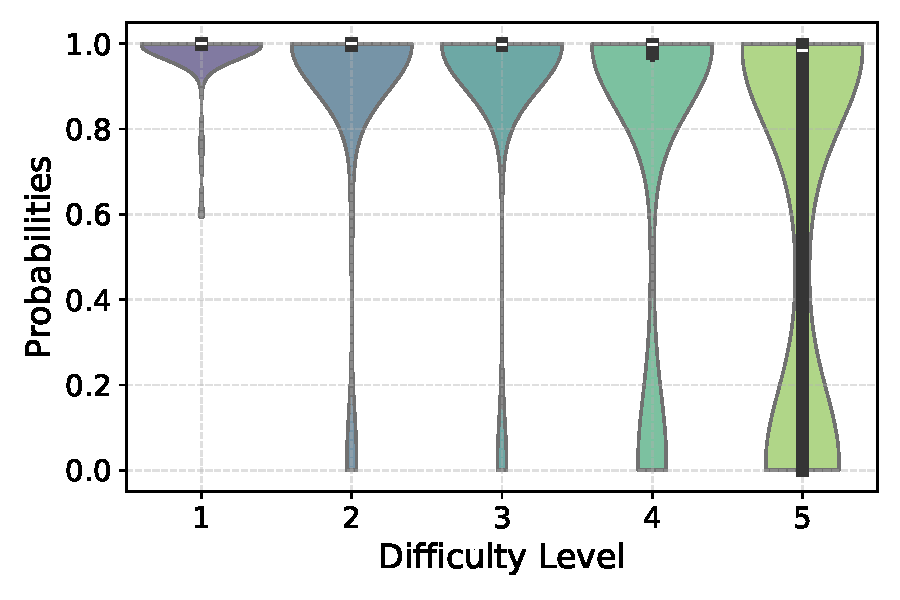
\includegraphics[width=\textwidth]{figs/QWEN-MATH-1.5B_violin_maj100_probability_adaptive_01_NO_ground_truth.pdf}
        \caption{Qwen2.5-Math-1.5B, $N_{\text{budget}}=100$.}
      \label{fig:QWEN-MATH-1.5B_budget_100_NO_01}
  \end{subfigure}
  \hfill
  \begin{subfigure}{0.49\textwidth}
      \centering
      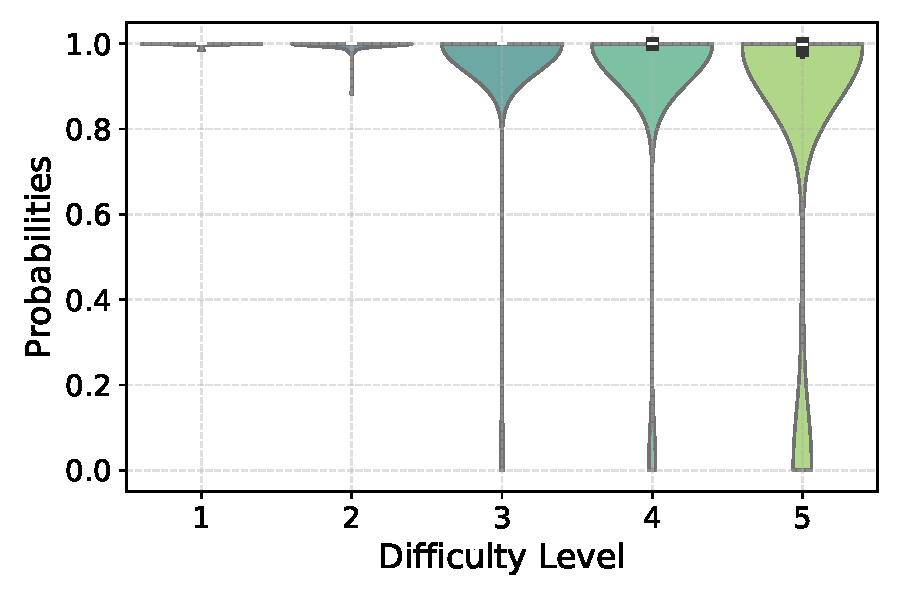
\includegraphics[width=\textwidth]{figs/QWEN-MATH-7B_violin_maj100_probability_adaptive_01_NO_ground_truth.pdf}
        \caption{Qwen2.5-Math-7B, $N_{\text{budget}}=100$.}
      \label{fig:QWEN-MATH-7B_budget_100_NO_01}
  \end{subfigure}
  \caption{Violin plots illustrating the distribution of the estimated lower bound on the probability $\mathbb{P}[\widehat{c}_n = c^\star]$ when applying Martingale Majority Certificate stopping rule with $\varepsilon = 0.1$ across different budget values $N_{\text{budget}}$. 
  Results are obtained after test-time training with SNR-based rewards on the MATH-500 dataset.}
  \label{fig:violin_plots_NO_ground_truth_01}
\end{figure}

\begin{figure}[h!]
  \centering
  \begin{subfigure}{0.49\textwidth}
      \centering
      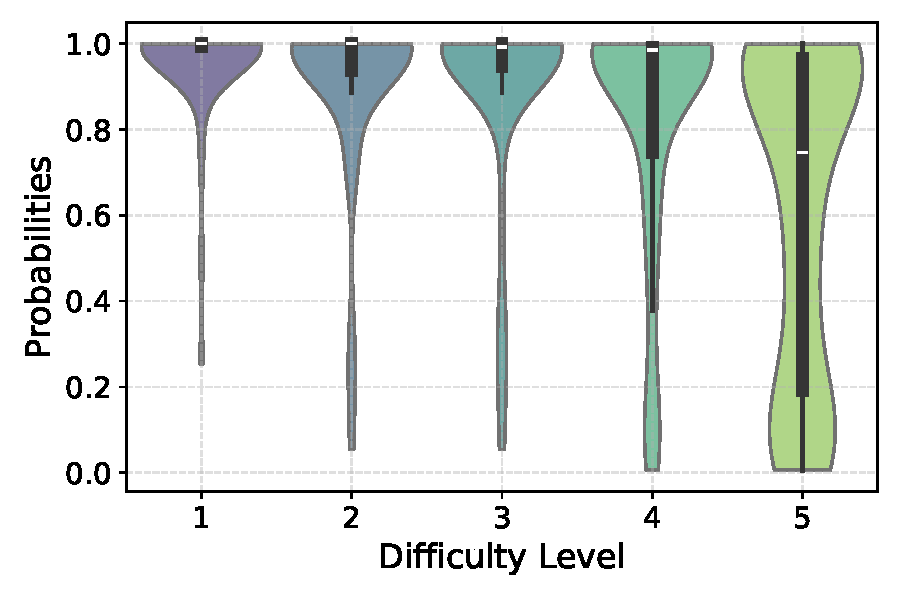
\includegraphics[width=\textwidth]{figs/QWEN-MATH-1.5B_violin_maj10_probability_adaptive_04_NO_ground_truth.pdf}
      \caption{Qwen2.5-Math-1.5B, $N_{\text{budget}}=10$.}
      \label{fig:QWEN-MATH-1.5B_budget_10_NO_04}
  \end{subfigure}
  \hfill
  \begin{subfigure}{0.49\textwidth}
      \centering
      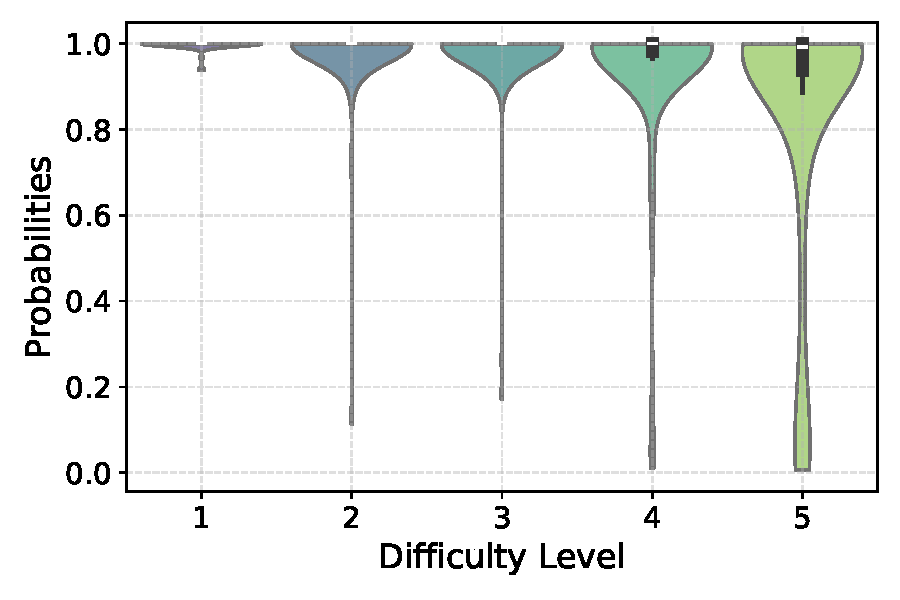
\includegraphics[width=\textwidth]{figs/QWEN-MATH-7B_violin_maj10_probability_adaptive_04_NO_ground_truth.pdf}
        \caption{Qwen2.5-Math-7B, $N_{\text{budget}}=10$.}
      \label{fig:QWEN-MATH-7B_budget_10_NO_04}
  \end{subfigure}
  \vfill
  \begin{subfigure}{0.49\textwidth}
      \centering
      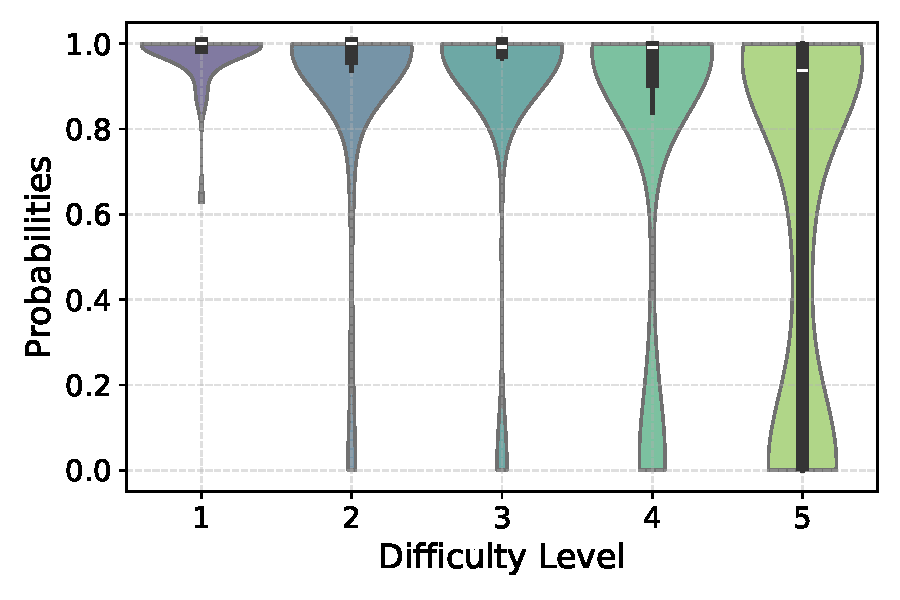
\includegraphics[width=\textwidth]{figs/QWEN-MATH-1.5B_violin_maj50_probability_adaptive_04_NO_ground_truth.pdf}
        \caption{Qwen2.5-Math-1.5B, $N_{\text{budget}}=50$.}
      \label{fig:QWEN-MATH-1.5B_budget_50_NO_04}
  \end{subfigure}
  \hfill
  \begin{subfigure}{0.49\textwidth}
      \centering
      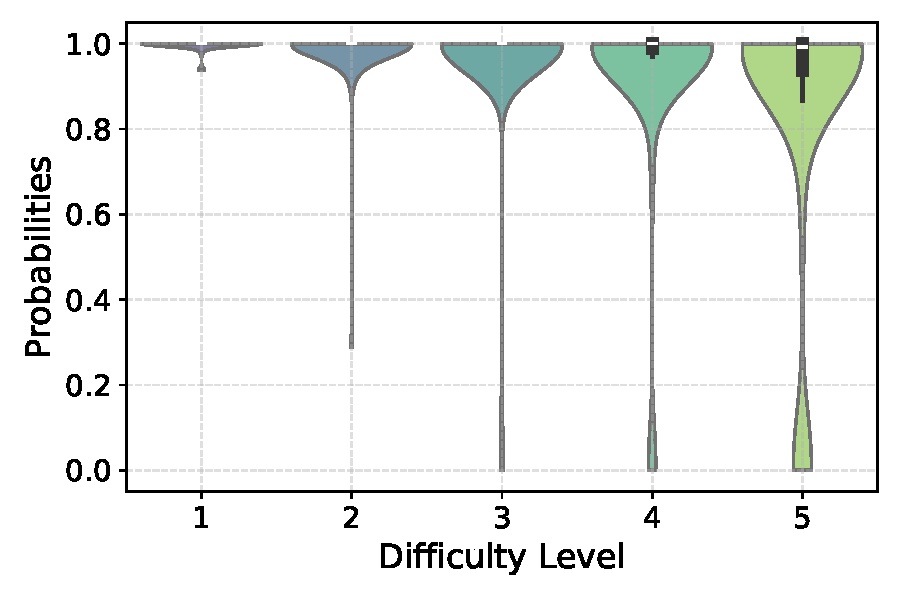
\includegraphics[width=\textwidth]{figs/QWEN-MATH-7B_violin_maj50_probability_adaptive_04_NO_ground_truth.pdf}
        \caption{Qwen2.5-Math-7B, $N_{\text{budget}}=50$.}
      \label{fig:QWEN-MATH-7B_budget_50_NO_04}
  \end{subfigure}
  \vfill
  \begin{subfigure}{0.49\textwidth}
      \centering
      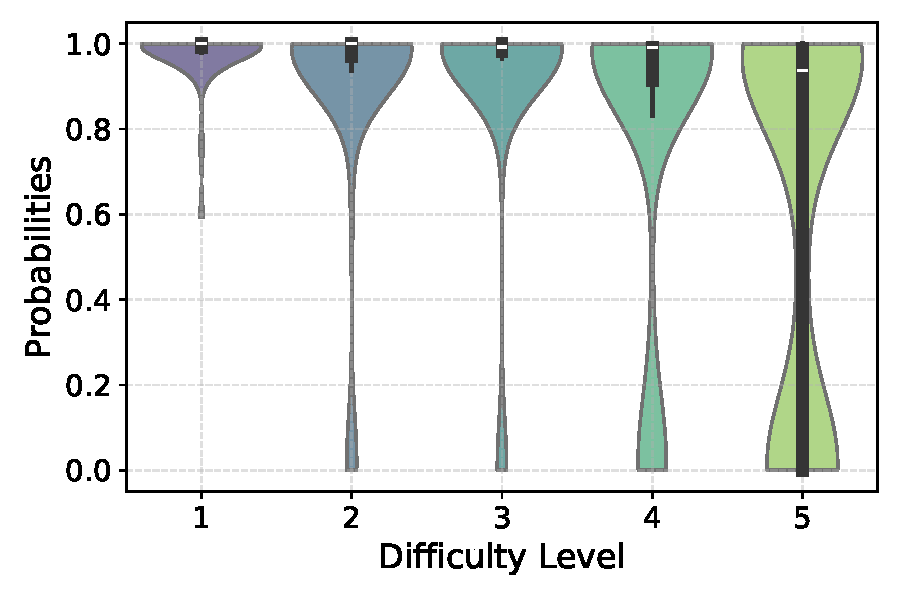
\includegraphics[width=\textwidth]{figs/QWEN-MATH-1.5B_violin_maj100_probability_adaptive_04_NO_ground_truth.pdf}
        \caption{Qwen2.5-Math-1.5B, $N_{\text{budget}}=100$.}
      \label{fig:QWEN-MATH-1.5B_budget_100_NO_04}
  \end{subfigure}
  \hfill
  \begin{subfigure}{0.49\textwidth}
      \centering
      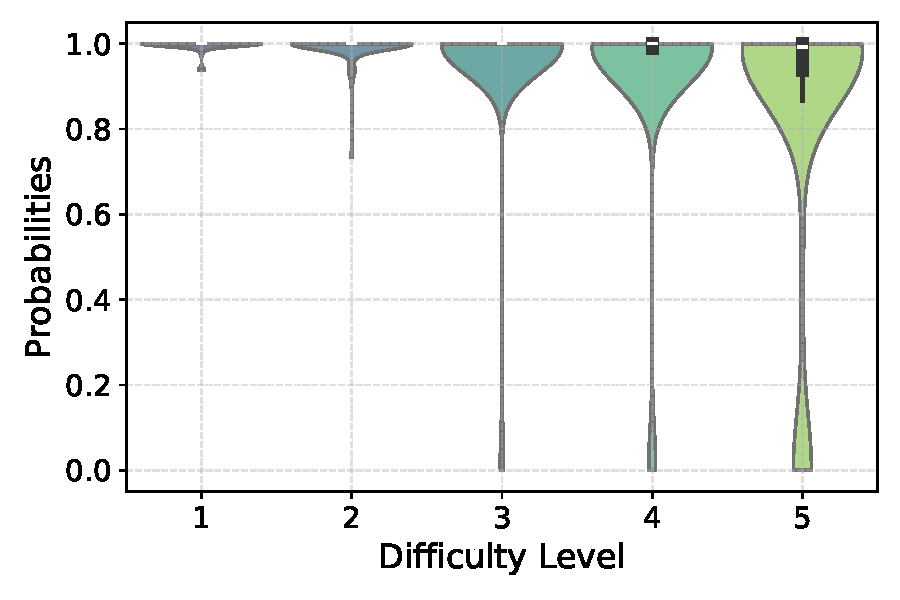
\includegraphics[width=\textwidth]{figs/QWEN-MATH-7B_violin_maj100_probability_adaptive_04_NO_ground_truth.pdf}
        \caption{Qwen2.5-Math-7B, $N_{\text{budget}}=100$.}
      \label{fig:QWEN-MATH-7B_budget_100_NO_04}
  \end{subfigure}
  \caption{Violin plots illustrating the distribution of the estimated lower bound on the probability $\mathbb{P}[\widehat{c}_n = c^\star]$ when applying Martingale Majority Certificate stopping rule with $\varepsilon = 0.4$ across different budget values $N_{\text{budget}}$. 
   Results are obtained after test-time training with SNR-based rewards on the MATH-500 dataset.}
  \label{fig:violin_plots_NO_ground_truth_04}
\end{figure}


\begin{figure}[h!]
  \centering
  \begin{subfigure}{0.49\textwidth}
      \centering
      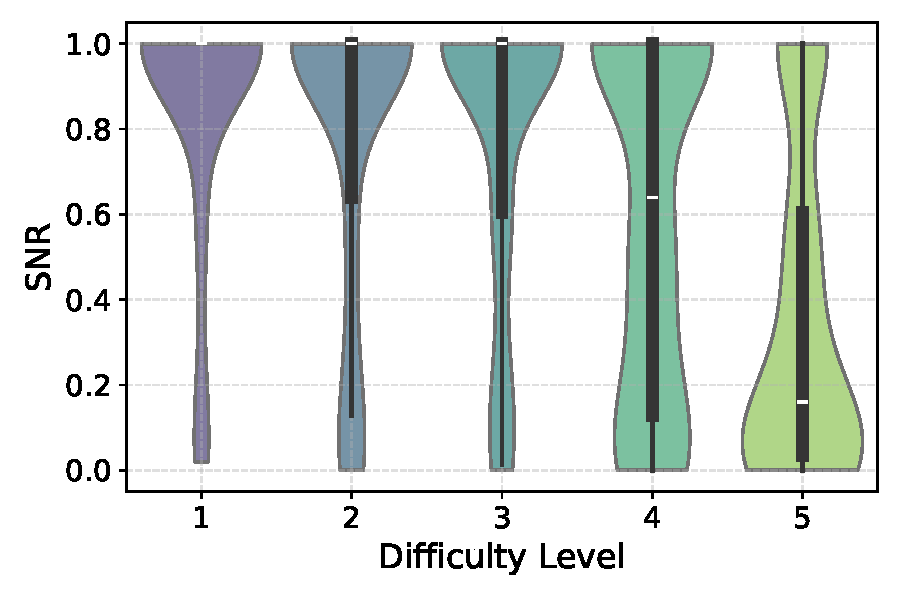
\includegraphics[width=\textwidth]{figs/QWEN-MATH-1.5B_violin_maj10_SNR_01.pdf}
      \caption{Qwen2.5-Math-1.5B, $N_{\text{budget}}=10$.}
      \label{fig:QWEN-MATH-1.5B_budget_10_SNR_01}
  \end{subfigure}
  \hfill
  \begin{subfigure}{0.49\textwidth}
      \centering
      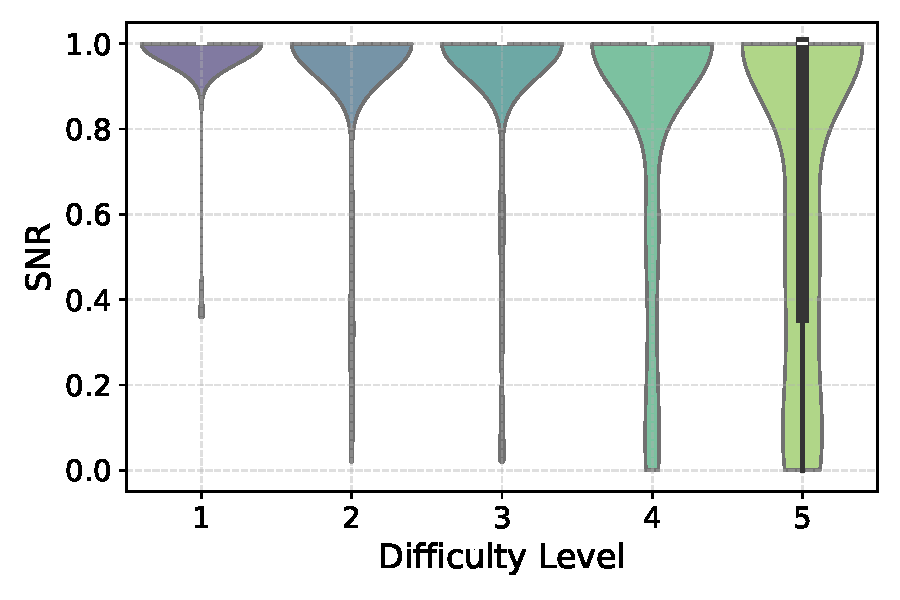
\includegraphics[width=\textwidth]{figs/QWEN-MATH-7B_violin_maj10_SNR_01.pdf}
        \caption{Qwen2.5-Math-7B, $N_{\text{budget}}=10$.}
      \label{fig:QWEN-MATH-7B_budget_10_SNR_01}
  \end{subfigure}
  \vfill
  \begin{subfigure}{0.49\textwidth}
      \centering
      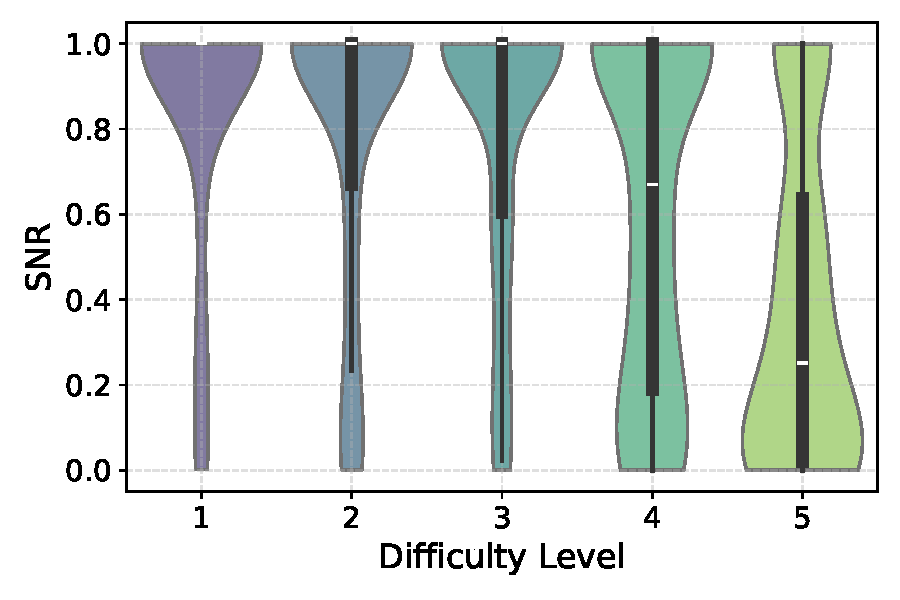
\includegraphics[width=\textwidth]{figs/QWEN-MATH-1.5B_violin_maj50_SNR_01.pdf}
        \caption{Qwen2.5-Math-1.5B, $N_{\text{budget}}=50$.}
      \label{fig:QWEN-MATH-1.5B_budget_50_SNR_01}
  \end{subfigure}
  \hfill
  \begin{subfigure}{0.49\textwidth}
      \centering
      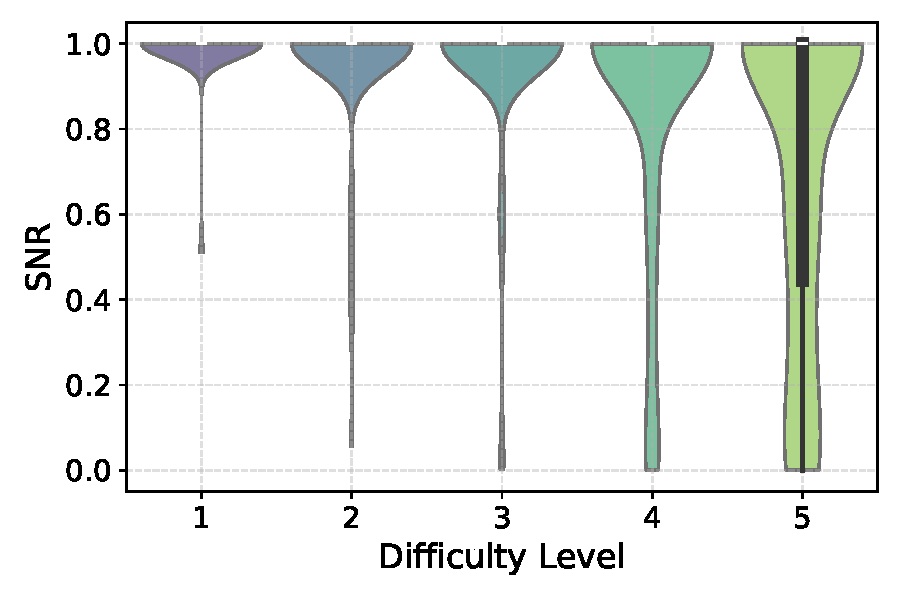
\includegraphics[width=\textwidth]{figs/QWEN-MATH-7B_violin_maj50_SNR_01.pdf}
        \caption{Qwen2.5-Math-7B, $N_{\text{budget}}=50$.}
      \label{fig:QWEN-MATH-7B_budget_50_SNR_01}
  \end{subfigure}
  \vfill
  \begin{subfigure}{0.49\textwidth}
      \centering
      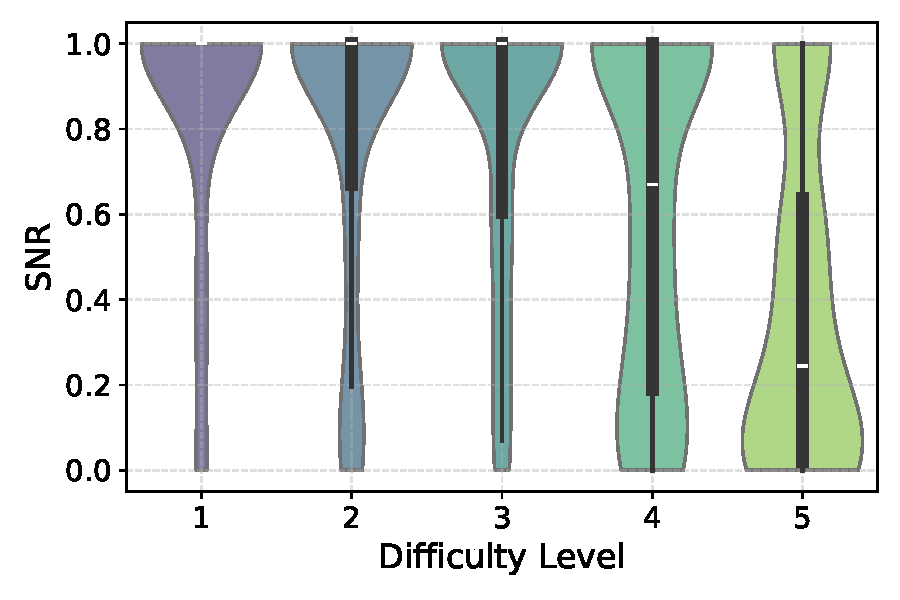
\includegraphics[width=\textwidth]{figs/QWEN-MATH-1.5B_violin_maj100_SNR_01.pdf}
        \caption{Qwen2.5-Math-1.5B, $N_{\text{budget}}=100$.}
      \label{fig:QWEN-MATH-1.5B_budget_100_SNR_01}
  \end{subfigure}
  \hfill
  \begin{subfigure}{0.49\textwidth}
      \centering
      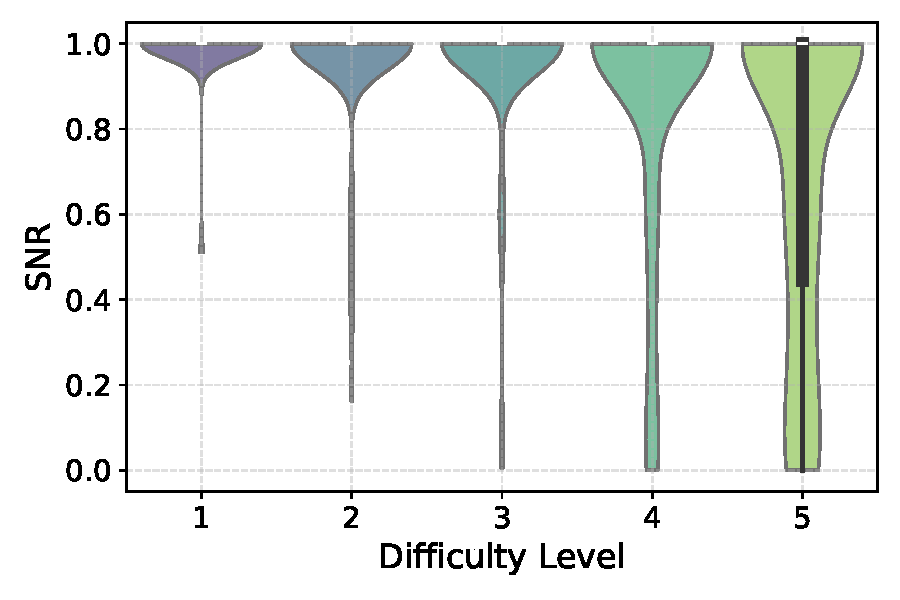
\includegraphics[width=\textwidth]{figs/QWEN-MATH-7B_violin_maj100_SNR_01.pdf}
        \caption{Qwen2.5-Math-7B, $N_{\text{budget}}=100$.}
      \label{fig:QWEN-MATH-7B_budget_100_SNR_01}
  \end{subfigure}
  \caption{Violin plots showing the distribution of the estimated signal-to-noise ratio between the leader and runner-up, $\text{SNR}(\Delta_{j^\star_n})$, when using Martingale Majority Certificate stopping rule with $\varepsilon = 0.1$ across different budget values $N_{\text{budget}}$. Results are obtained after applying test-time training with SNR-based rewards on the MATH-500 dataset.}
  \label{fig:violin_plots_SNR_ground_truth_01}
\end{figure}

\begin{figure}[h!]
  \centering
  \begin{subfigure}{0.49\textwidth}
      \centering
      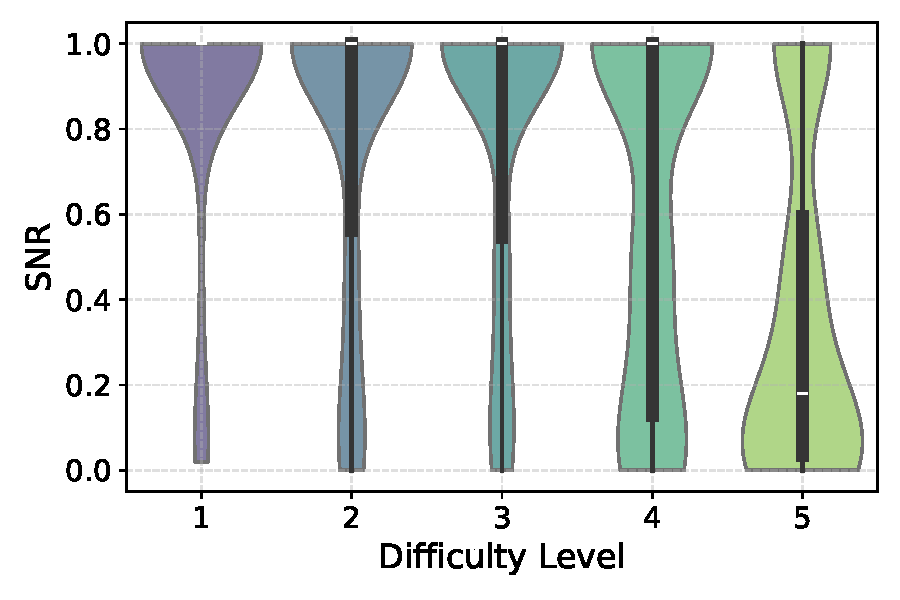
\includegraphics[width=\textwidth]{figs/QWEN-MATH-1.5B_violin_maj10_SNR_04.pdf}
      \caption{Qwen2.5-Math-1.5B, $N_{\text{budget}}=10$.}
      \label{fig:QWEN-MATH-1.5B_budget_10_SNR_04}
  \end{subfigure}
  \hfill
  \begin{subfigure}{0.49\textwidth}
      \centering
      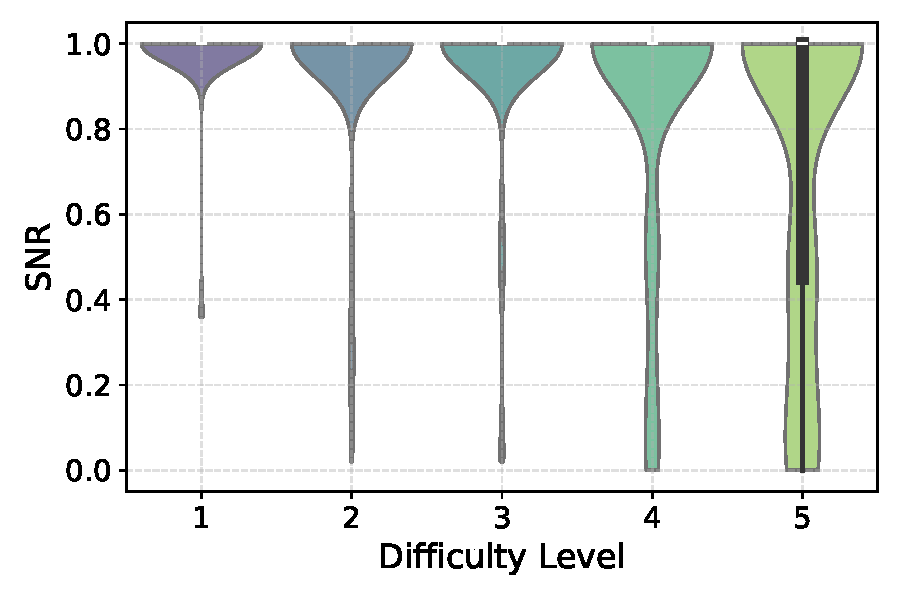
\includegraphics[width=\textwidth]{figs/QWEN-MATH-7B_violin_maj10_SNR_04.pdf}
        \caption{Qwen2.5-Math-7B, $N_{\text{budget}}=10$.}
      \label{fig:QWEN-MATH-7B_budget_10_SNR_04}
  \end{subfigure}
  \vfill
  \begin{subfigure}{0.49\textwidth}
      \centering
      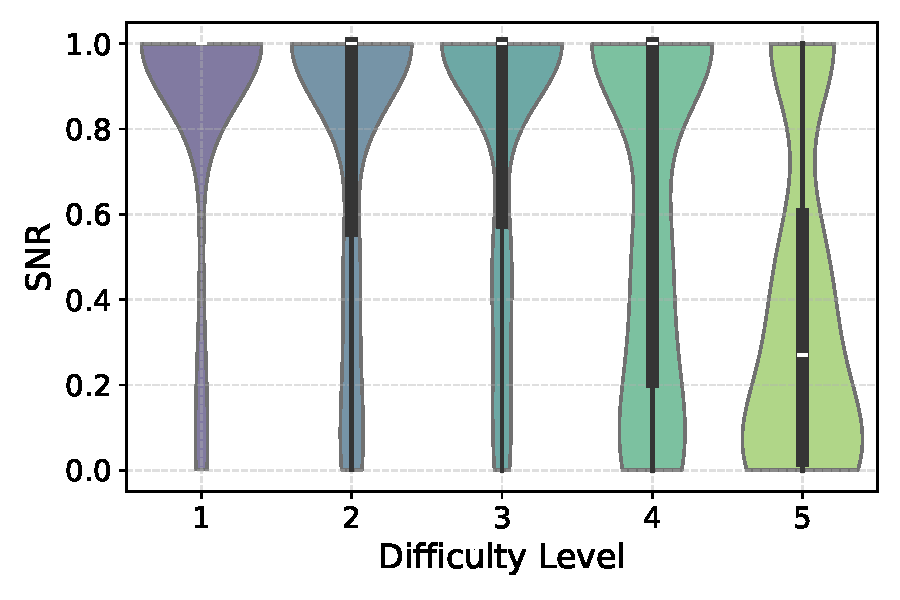
\includegraphics[width=\textwidth]{figs/QWEN-MATH-1.5B_violin_maj50_SNR_04.pdf}
        \caption{Qwen2.5-Math-1.5B, $N_{\text{budget}}=50$.}
      \label{fig:QWEN-MATH-1.5B_budget_50_SNR_04}
  \end{subfigure}
  \hfill
  \begin{subfigure}{0.49\textwidth}
      \centering
      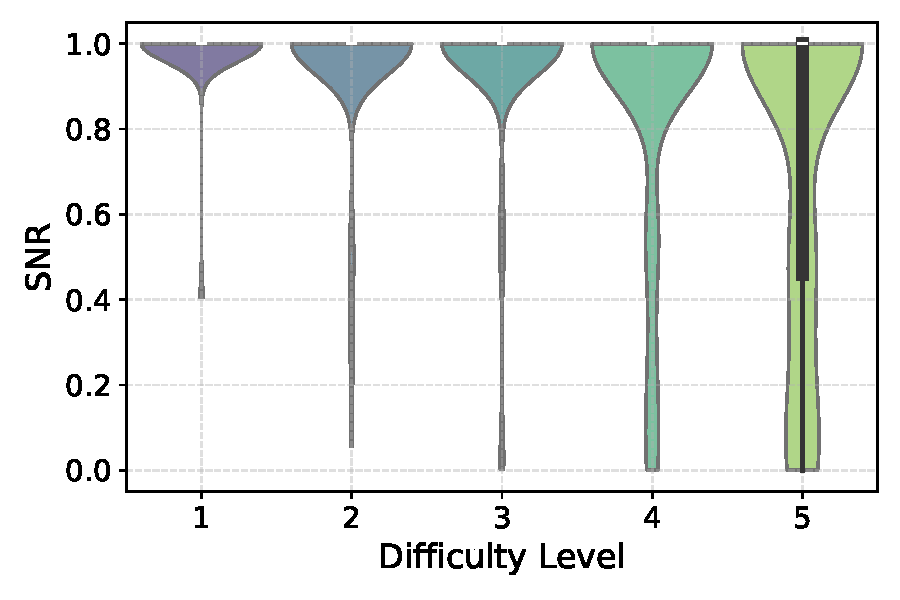
\includegraphics[width=\textwidth]{figs/QWEN-MATH-7B_violin_maj50_SNR_04.pdf}
        \caption{Qwen2.5-Math-7B, $N_{\text{budget}}=50$.}
      \label{fig:QWEN-MATH-7B_budget_50_SNR_04}
  \end{subfigure}
  \vfill
  \begin{subfigure}{0.49\textwidth}
      \centering
      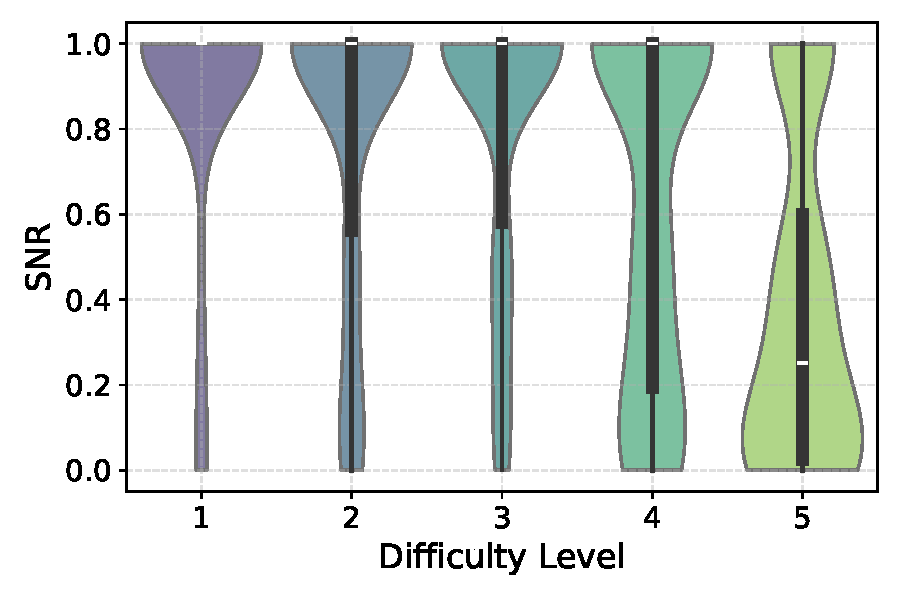
\includegraphics[width=\textwidth]{figs/QWEN-MATH-1.5B_violin_maj100_SNR_04.pdf}
        \caption{Qwen2.5-Math-1.5B, $N_{\text{budget}}=100$.}
      \label{fig:QWEN-MATH-1.5B_budget_100_SNR_04}
  \end{subfigure}
  \hfill
  \begin{subfigure}{0.49\textwidth}
      \centering
      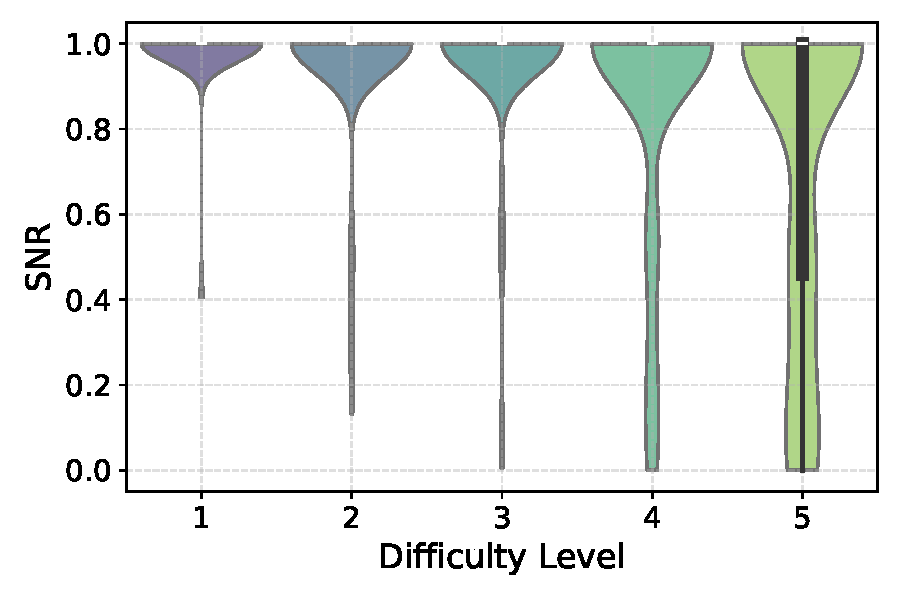
\includegraphics[width=\textwidth]{figs/QWEN-MATH-7B_violin_maj100_SNR_04.pdf}
        \caption{Qwen2.5-Math-7B, $N_{\text{budget}}=100$.}
      \label{fig:QWEN-MATH-7B_budget_100_SNR_04}
  \end{subfigure}
  \caption{Violin plots showing the distribution of the estimated signal-to-noise ratio between the leader and runner-up, ${\text{SNR}}(\Delta_{j^\star_n})$, when using Martingale Majority Certificate stopping rule with $\varepsilon = 0.4$ across different budget values $N_{\text{budget}}$. Results are obtained after applying test-time training with SNR-based rewards on the MATH-500 dataset.}
  \label{fig:violin_plots_SNR_ground_truth_04}
\end{figure}
